\section{Results}
\label{sec:results}

\subsection{Where the Baseline Loses Accuracy}
\label{sec:gap}

To know what a component could gain, we first located the baseline's errors
on ImageNet-R (Table~\ref{tab:gap}).
\begin{itemize}
  \item \emph{Gap to joint training.} Training once on all 200 classes gives
    $A_B=86.52$, which is $3.9$ points above the baseline.
  \item \emph{The gap sits in the oldest classes.} Tasks~0 and~1 lose $9.0$
    and $8.3$ points, while the newest task matches joint training.
  \item \emph{The extra errors are cross-task.} Per pair of classes, the
    ratio of cross-task to within-task confusions is $1.38$ for the baseline
    and $0.90$ for joint training.
  \item \emph{Exact statistics do not close the gap.} Giving the classifier
    alignment the oracle statistics of old classes, recomputed from their
    images, adds only $+0.195$ to $\bar A$. It lifts task~0 from $80.1$ to
    $87.1$, but newer tasks drop, because their classes are now predicted as
    task~0 more often.
\end{itemize}
The remaining errors are therefore overlaps between tasks in the learned
representation. An inference-time component can at best arbitrate between
tasks better. This is the target of the hierarchical measurement and of the
fusion.

\begin{table}[t]
\centering
\caption{Final accuracy (\%) per task on ImageNet-R; task 0 holds the oldest
classes. CIL: baseline, 4 replicates. Oracle: classifier alignment with
exact old-class statistics, 2 runs. Joint: one task with all 200 classes.}
\label{tab:gap}
\setlength{\tabcolsep}{4pt}
\begin{adjustbox}{max width=\textwidth}
\begin{tabular}{lrrrrrrrrrr}
\toprule
Task & 0 & 1 & 2 & 3 & 4 & 5 & 6 & 7 & 8 & 9\\
\midrule
Joint  & 89.1 & 88.7 & 86.4 & 86.4 & 83.2 & 86.0 & 85.8 & 87.0 & 85.4 & 85.8\\
CIL    & 80.1 & 80.4 & 82.7 & 82.3 & 78.8 & 82.7 & 85.3 & 84.2 & 83.9 & 86.2\\
Oracle & 87.1 & 83.1 & 83.5 & 82.2 & 79.1 & 81.6 & 84.7 & 82.9 & 82.1 & 83.6\\
\midrule
Joint $-$ CIL & $+9.0$ & $+8.3$ & $+3.7$ & $+4.1$ & $+4.4$ & $+3.3$ & $+0.5$ & $+2.9$ & $+1.6$ & $-0.3$\\
\bottomrule
\end{tabular}
\end{adjustbox}
\end{table}

\subsection{Quantum Components against their Classical Twins}

\begin{table}[t]
\centering
\caption{Every quantum placement against its classical twin. $\Delta\bar A$ in
points with 95\% CI over paired runs; $n$ is the number of runs.
R: ImageNet-R, A: ImageNet-A.}
\label{tab:quantum}
\setlength{\tabcolsep}{3pt}
\begin{adjustbox}{max width=\textwidth}
\begin{tabular}{llll}
\toprule
Placement & Comparison & $\Delta\bar A$ [95\% CI] & $n$ \\
\midrule
1. PQK, steering metric & PQK $-$ cosine (baseline), R & $+0.06$ [$-0.07$, $+0.18$] & 3 \\
2. PQK, separation metric & current $-$ previous features, R & $-0.02$ [$-0.06$, $+0.03$] & 3 \\
\multirow{4}{*}{3. PQK, feature map} & PQK ridge $-$ linear head, A & $-17.33$ [$-19.07$, $-15.59$] & 3 \\
 & PQK without CNOTs $-$ linear head, A & $-10.40$ [$-11.10$, $-9.71$] & 3 \\
 & random Fourier features $-$ linear head, A & $-1.41$ [$-2.52$, $-0.31$] & 3 \\
 & random projection $-$ linear head, A & $-1.24$ [$-2.29$, $-0.19$] & 3 \\
\midrule
\multirow{4}{*}{4. PGM, stand-alone} & PGM $-$ ridge, same statistics, R+A & $+0.09$ [$-0.23$, $+0.40$] & 11 \\
 & moment states $-$ per-sample states, R+A & $+0.07$ [$-0.02$, $+0.16$] & 11 \\
 & transport channel $-$ no transport, R & $-0.03$ [$-0.19$, $+0.14$] & 5 \\
 & two-copy encoding $-$ amplitude encoding & $-3.6$ (R), $-6.5$ (A) & 5+5 \\
5. PGM, fused & SCF-PGM $-$ SCF-ridge, 4 datasets & $-0.04$ [$-0.17$, $+0.08$] & 12 \\
\bottomrule
\end{tabular}
\end{adjustbox}
\end{table}

Table~\ref{tab:quantum} is the main result of this study.
\begin{itemize}
  \item \emph{No quantum component beats its twin.} Every 95\% interval
    either contains zero or lies below it.
  \item \emph{Two placements are clearly harmful:} the PQK as a feature map,
    and the richer two-copy encoding.
  \item \emph{The measurement placements match theory.} The PGM matches
    ridge on the same statistics, alone and fused, as the least-squares
    equivalence and Propositions~\ref{prop:unitary}--\ref{prop:shrink}
    suggest.
\end{itemize}

\subsection{Mechanisms}

\paragraph{Kernel: local reduced states concentrate.}
\begin{itemize}
  \item \emph{As a steering or separation metric}, the frozen 8-qubit kernel
    rates almost every pair of prototype and feature as similar,
    $k\approx0.5$--$0.6$. The separation term stays at about $0.45$
    throughout training: the adapter, constrained by its alignment loss,
    never reduces the quantum similarity through the 8-dimensional
    bottleneck.
  \item \emph{As a feature map}, two effects compound.
    \begin{itemize}
      \item The classifier-alignment pseudo-data are degenerate. With about
        30 images per class, each covariance has rank at most 29. The
        Gaussian samples are then trivially separable: random Fourier
        features reach $100\%$ on held-out pseudo-data but only about $67\%$
        on real test images.
      \item The PQK cannot even fit this easy problem. It reaches $78$--$91\%$
        on held-out pseudo-data, $88$--$96\%$ without CNOTs. After random
        CNOT layers, information moves into non-local correlations, and the
        one-qubit states drift towards the maximally mixed state.
    \end{itemize}
    The kernel--target alignment confirms this: $0.34$ for the PQK, against
    $0.37$ (random Fourier features), $0.38$ (random projection) and $0.38$
    (PQK without CNOTs).
\end{itemize}

\paragraph{Measurement: competitive at first, then overtaken by drift.}
\begin{itemize}
  \item \emph{In the base task}, where there is no drift, the PGM matches
    the linear head on ImageNet-R ($-0.31$, $[-0.77,+0.15]$), beats it on
    ImageNet-A ($+1.57$), and beats ridge on the same statistics on
    ImageNet-R ($+0.68$, $[+0.44,+0.92]$).
  \item \emph{As tasks accumulate}, its deficit to the linear head grows
    linearly, from $-0.31$ to $-2.79$ on ImageNet-R. The extra errors are
    old images assigned to newer tasks: $11.5\%$ of the test set, against
    $9.9\%$ for the linear head.
  \item \emph{Better states do not remove the deficit:}
    \begin{itemize}
      \item transporting the states by a fitted channel changes nothing
        (Table~\ref{tab:quantum}), although the channel deviates from the
        identity by about $8\%$ per task;
      \item building them from drift-corrected rather than stale means gains
        only $+0.13$;
      \item oracle states, recomputed from old images, lift task~0 by
        $2.8$--$6.5$ points but $A_B$ by only $+0.64$.
    \end{itemize}
  \item \emph{The hierarchical measurement removes about two thirds} of the
    growing deficit, by arbitrating between tasks first: $+0.33$
    ($[+0.02,+0.64]$) over the flat PGM. It still stays below the linear head.
  \item \emph{Regularisation.} Decreasing $\delta$ tenfold changes accuracy by
    less than $0.3$ points; increasing it tenfold costs about $0.7$.
  \item \emph{The two-copy encoding} is already $2.5$ points below the linear
    head in the base task on ImageNet-R, so its failure is not due to drift.
    It adds dimensions that the class statistics cannot support.
\end{itemize}

\subsection{Measurement Fusion}
\label{sec:fusion-results}

Stand-alone, every generative score is worse than the linear head. The two,
however, err on different images. On ImageNet-R they disagree on $14\%$ of
the test images: the linear head is right on $5.8\%$ of them, the PGM on
$3.2\%$, and neither on $5.4\%$. Fusion (Eq.~\ref{eq:fusion}) exploits this.

\paragraph{Calibration is essential.}
An uncalibrated sum of the classifier log-softmax and the PGM
log-probabilities follows the linear head on $87\%$ of the disagreements,
because Born probabilities are much flatter than a softmax at scale $s$.
That uncalibrated sum gains only $+0.25$ (ImageNet-R) and $+0.44$
(ImageNet-A). The scale $\kappa$ removes this imbalance.

\begin{table}[t]
\centering
\caption{Fusion on four benchmarks, mean $\pm$ SD over seeds 1993, 2015 and
2026; $\Delta$: paired difference to the baseline in the same runs, with 95\%
CI. Weights were frozen on ImageNet-R (ridge $w=0.25$, PGM $w=0.5$). Grey:
published baseline numbers (one seed, the authors' partitions).}
\label{tab:main}
\setlength{\tabcolsep}{2.2pt}
\renewcommand{\arraystretch}{1.1}
\resizebox{\textwidth}{!}{%
\begin{tabular}{lcccccccccc}
\toprule
& \multicolumn{2}{c}{CIFAR-100} & \multicolumn{2}{c}{ImageNet-R} & \multicolumn{2}{c}{ImageNet-A}
& \multicolumn{2}{c}{CUB-200} & \multicolumn{2}{c}{Average} \\
\cmidrule(lr){2-3}\cmidrule(lr){4-5}\cmidrule(lr){6-7}\cmidrule(lr){8-9}\cmidrule(lr){10-11}
Method & $\bar A$ & $A_B$ & $\bar A$ & $A_B$ & $\bar A$ & $A_B$ & $\bar A$ & $A_B$ & $\bar A$ & $A_B$ \\
\midrule
\rowcolor{gray!12}
Baseline~\cite{rsiat}, published & 95.15 & 92.20 & 86.92 & 82.75 & 74.89 & 66.23 & 93.99 & 90.59 & -- & -- \\
\midrule
Baseline (ours) & 95.02{\tiny$\pm$.21} & 92.03{\tiny$\pm$.19} & 87.11{\tiny$\pm$.49} & 82.55{\tiny$\pm$.05}
 & 74.26{\tiny$\pm$1.1} & 67.02{\tiny$\pm$1.1} & 93.53{\tiny$\pm$.79} & 88.47{\tiny$\pm$.31} & 87.48 & 82.52 \\
SCF, ridge (classical) & 95.22{\tiny$\pm$.20} & \textbf{92.41}{\tiny$\pm$.21} & 87.42{\tiny$\pm$.46} & 83.03{\tiny$\pm$.24}
 & \textbf{75.12}{\tiny$\pm$1.2} & \textbf{67.69}{\tiny$\pm$0.9} & \textbf{93.54}{\tiny$\pm$.88} & \textbf{88.85}{\tiny$\pm$.22} & \textbf{87.83} & \textbf{83.00} \\
SCF, PGM (quantum) & \textbf{95.23}{\tiny$\pm$.22} & 92.34{\tiny$\pm$.16} & \textbf{87.50}{\tiny$\pm$.43} & \textbf{83.07}{\tiny$\pm$.42}
 & 74.89{\tiny$\pm$1.0} & 67.65{\tiny$\pm$1.3} & 93.50{\tiny$\pm$.84} & 88.57{\tiny$\pm$.30} & 87.78 & 82.91 \\
\midrule
$\Delta$ ridge & $+$.20 {\tiny[.12,.28]} & $+$.38 {\tiny[.08,.69]} & $+$.32 {\tiny[.12,.51]} & $+$.48 {\tiny[.02,.94]}
 & $+$.85 {\tiny[.62,1.08]} & $+$.67 {\tiny[$-$.20,1.54]} & $+$.02 {\tiny[$-$.24,.27]} & $+$.38 {\tiny[.16,.61]} & $+$.35 & $+$.48 \\
$\Delta$ PGM & $+$.22 {\tiny[.15,.28]} & $+$.31 {\tiny[.18,.43]} & $+$.39 {\tiny[.25,.53]} & $+$.52 {\tiny[$-$.41,1.45]}
 & $+$.63 {\tiny[$-$.10,1.36]} & $+$.62 {\tiny[$-$.08,1.32]} & $-$.03 {\tiny[$-$.18,.12]} & $+$.10 {\tiny[.05,.16]} & $+$.30 & $+$.39 \\
\bottomrule
\end{tabular}}
\end{table}

\begin{figure}[t]
\centering
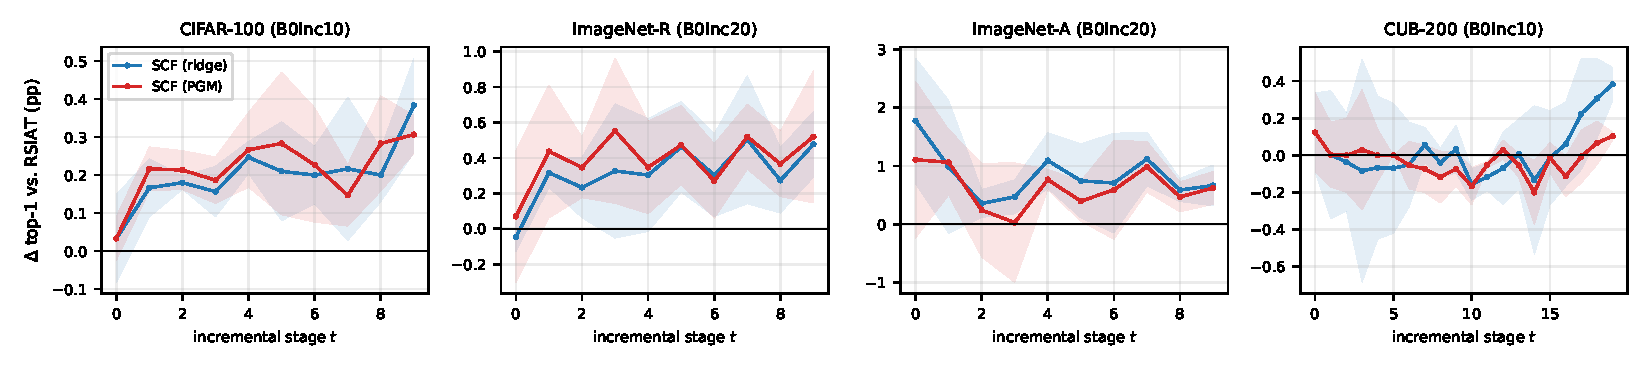
\includegraphics[width=\linewidth]{figures/delta_per_stage.pdf}
\caption{Paired gain of fusion over the baseline at each stage, mean $\pm$ SD
over three seeds. Blue: ridge source (classical). Red: PGM source (quantum).
The two sources track each other on every dataset.}
\label{fig:stage}
\end{figure}

\begin{table}[t]
\centering
\caption{Every pre-registered test, in the order it was run.}
\label{tab:tests}
\setlength{\tabcolsep}{3pt}
\begin{adjustbox}{max width=\textwidth}
\begin{tabular}{llll}
\toprule
Test & Runs & $\Delta$ [95\% CI] & Outcome \\
\midrule
SCF-PGM beats baseline by $\ge0.3$ $\bar A$, held-out & R, A; 8 & $+0.46$ [$+0.28$, $+0.64$] & passed \\
Transfer to unseen datasets, SCF-ridge & CIFAR, CUB; 6 & $+0.11$ [$-0.02$, $+0.24$] & \textbf{failed} \\
Transfer to unseen datasets, SCF-PGM & CIFAR, CUB; 6 & $+0.09$ [$-0.05$, $+0.24$] & \textbf{failed} \\
PGM better than ridge as fusion source & all; 12 & $-0.04$ [$-0.17$, $+0.08$] & \textbf{failed} \\
Oracle states worth $\ge1$ point of $A_B$ & R, A; 11 & $+0.64$ [$+0.48$, $+0.80$] & \textbf{failed} \\
\bottomrule
\end{tabular}
\end{adjustbox}
\end{table}

Table~\ref{tab:main} and Figure~\ref{fig:stage} give the fusion results, and
Table~\ref{tab:tests} the pre-registered tests.
\begin{itemize}
  \item \emph{Final accuracy rises on all four datasets}, by $+0.38$ to
    $+0.67$ with the ridge source. The CI excludes zero on three of them.
  \item \emph{Average accuracy rises on three:} CIFAR-100, ImageNet-R and
    ImageNet-A. It does not rise on CUB-200, where the gain appears only in
    the last 3 of 20 stages, and no weight in the grid helps. The
    pre-registered transfer test therefore failed.
  \item \emph{The number of images per class does not explain this.} CUB-200
    and ImageNet-A both have about 30 images per class and behave
    differently.
  \item \emph{Forgetting} falls on CUB-200 ($-0.57$), barely changes on
    CIFAR-100 and ImageNet-R, and rises on ImageNet-A ($+1.03$). There the
    fusion helps new classes more than old ones, $+1.60$ against $+0.53$,
    which raises each class's peak more than its final accuracy.
  \item \emph{Throughout, the quantum and classical sources are
    interchangeable.}
\end{itemize}
